\chapter{Scaling Your Practice with Automation}


\section{Introduction}

As an IT consultant, you've mastered the art of solving complex technical problems for your clients. But how do you take your practice to the next level? The answer lies in strategic automation. In this chapter, we'll explore how to create an automation roadmap, price your automated services effectively, and learn from a real-world case study of explosive growth through automation.


\section{Creating Your Automation Roadmap}

An automation roadmap is your strategic plan for implementing automation across your practice. Let's break down the process into manageable steps:

\subsection{Step 1: Identify Automation Candidates}

Begin by listing all the processes in your practice. Consider:
\begin{itemize}
    \item Client onboarding
    \item Project management
    \item Reporting and analytics
    \item Billing and invoicing
    \item Customer support
    \item Marketing and lead generation
\end{itemize}

\begin{figure}[h]
    \centering
    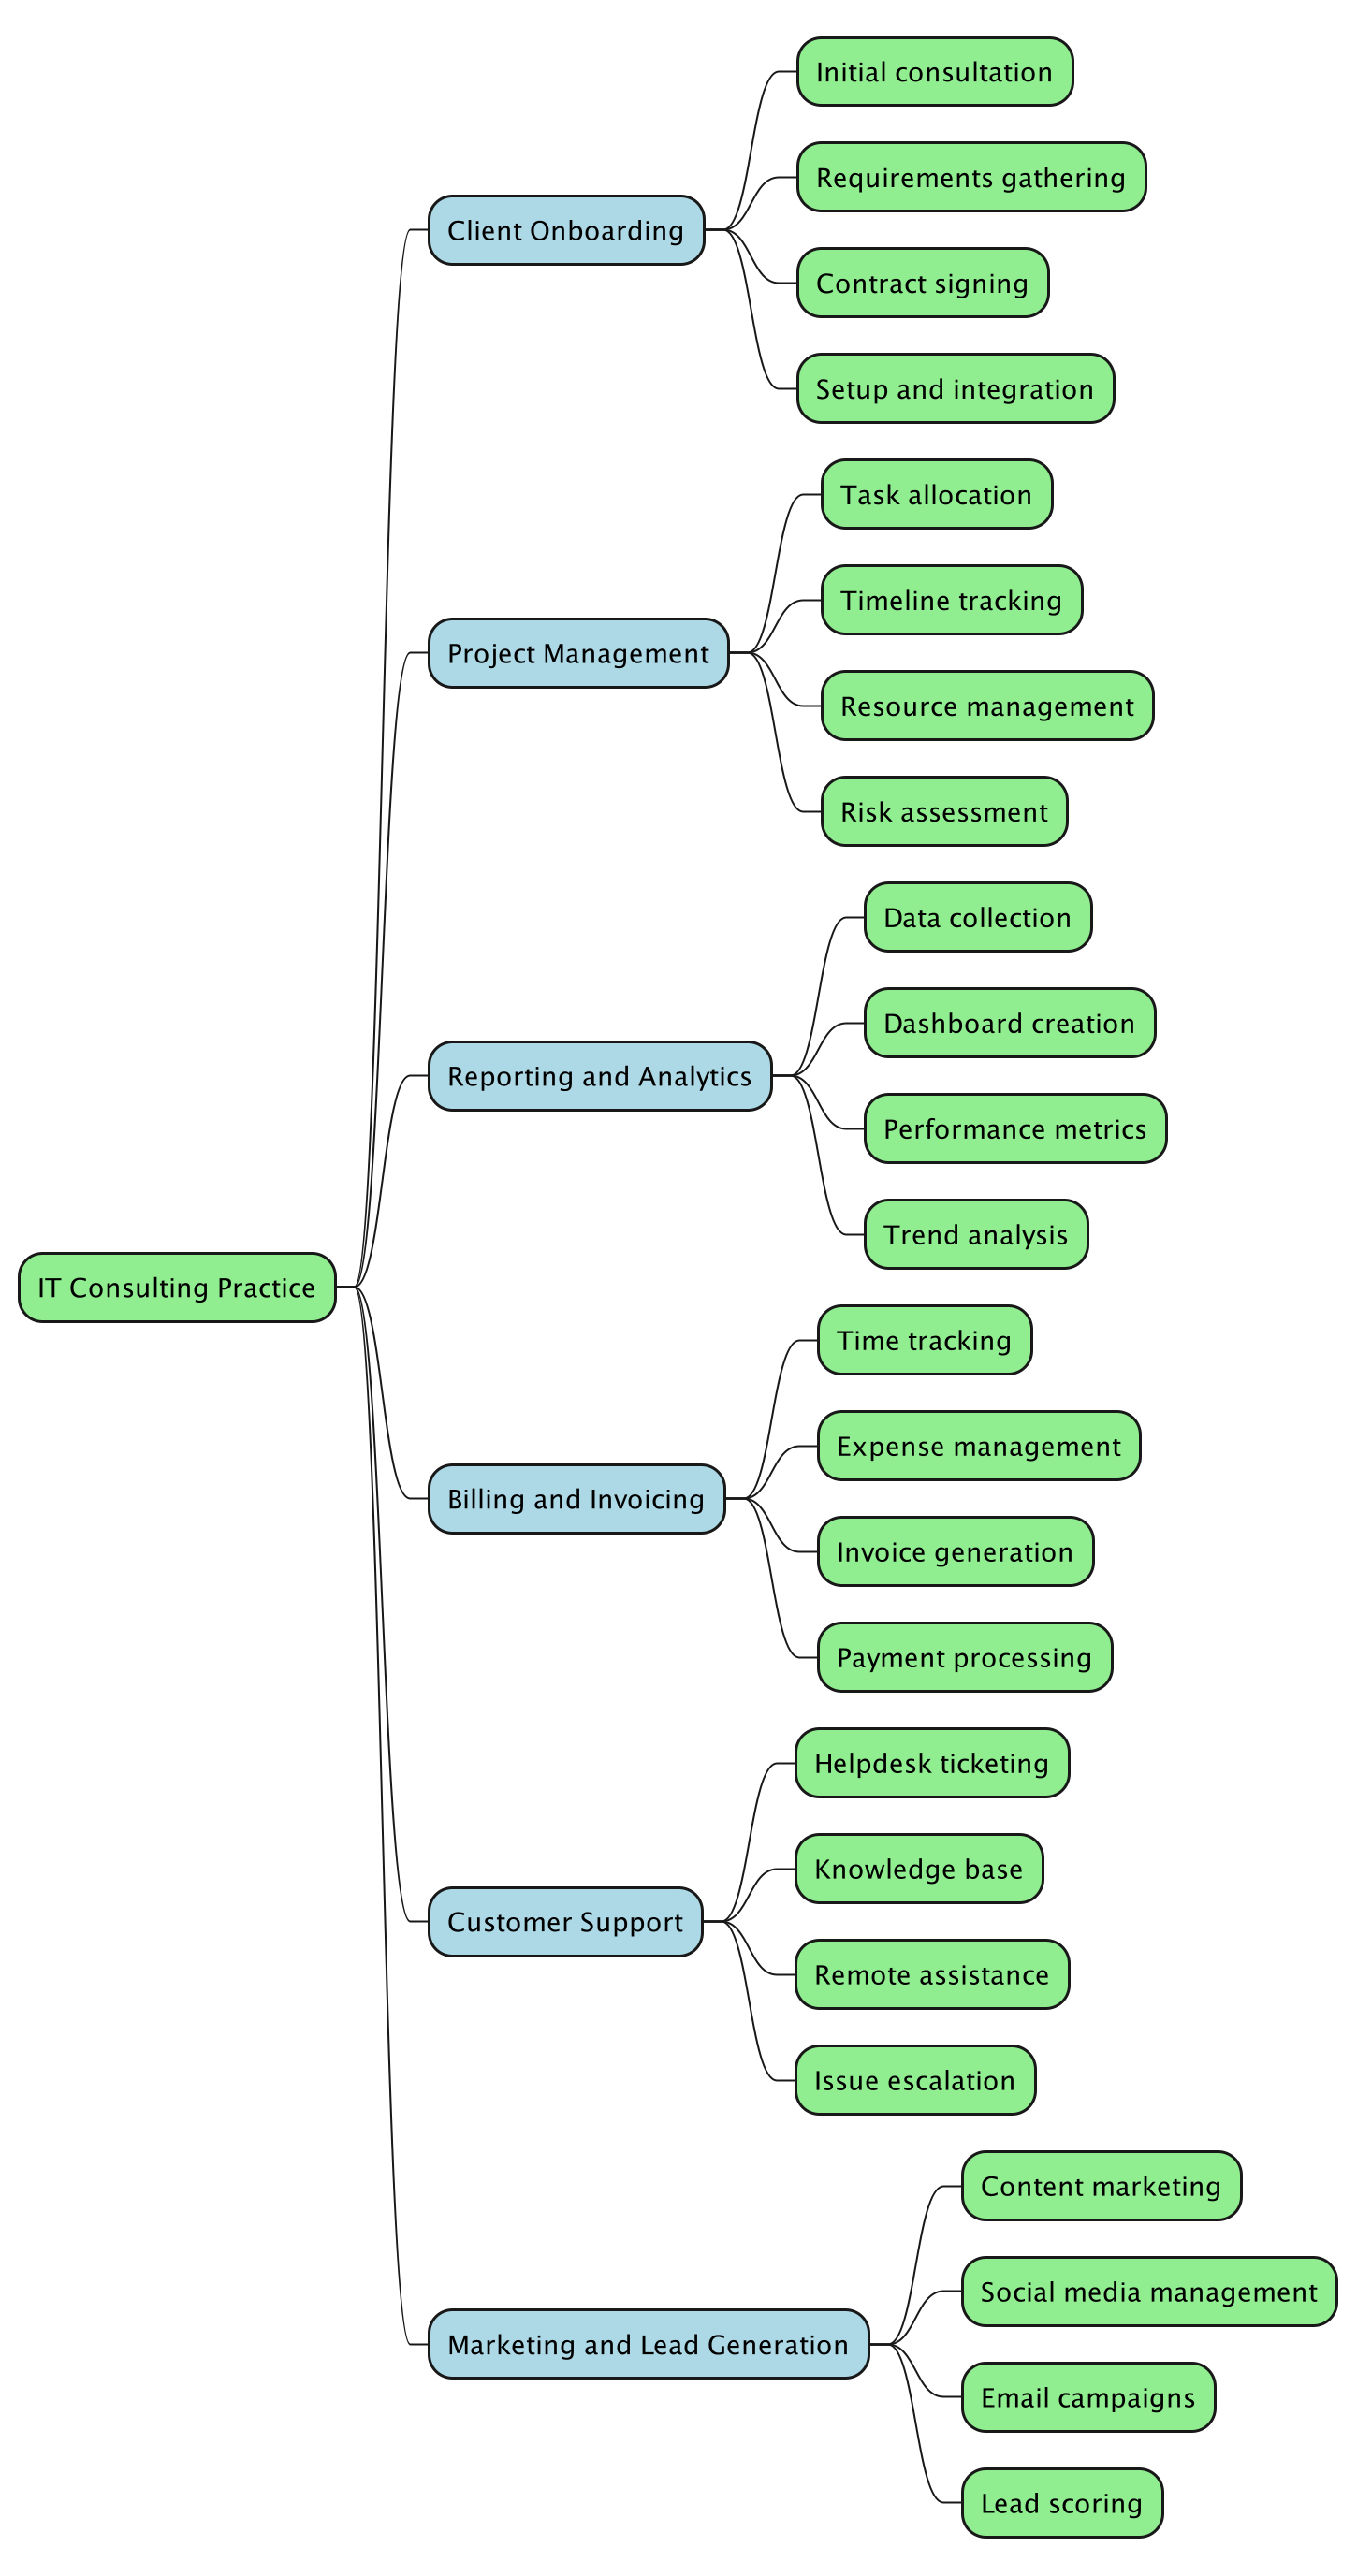
\includegraphics[width=0.40\textwidth]{./figures/04-consulting_practice_mindmap}
    \caption{Mind Map of IT Consulting Practice Areas}
    \label{fig:consulting_mindmap}
\end{figure}

\subsection{Step 2: Prioritize Processes}

Not all processes are created equal. Prioritize based on:
\begin{itemize}
    \item Potential time savings
    \item Impact on client satisfaction
    \item Complexity of automation
    \item Frequency of the process
\end{itemize}

Create a matrix to visualize priority:

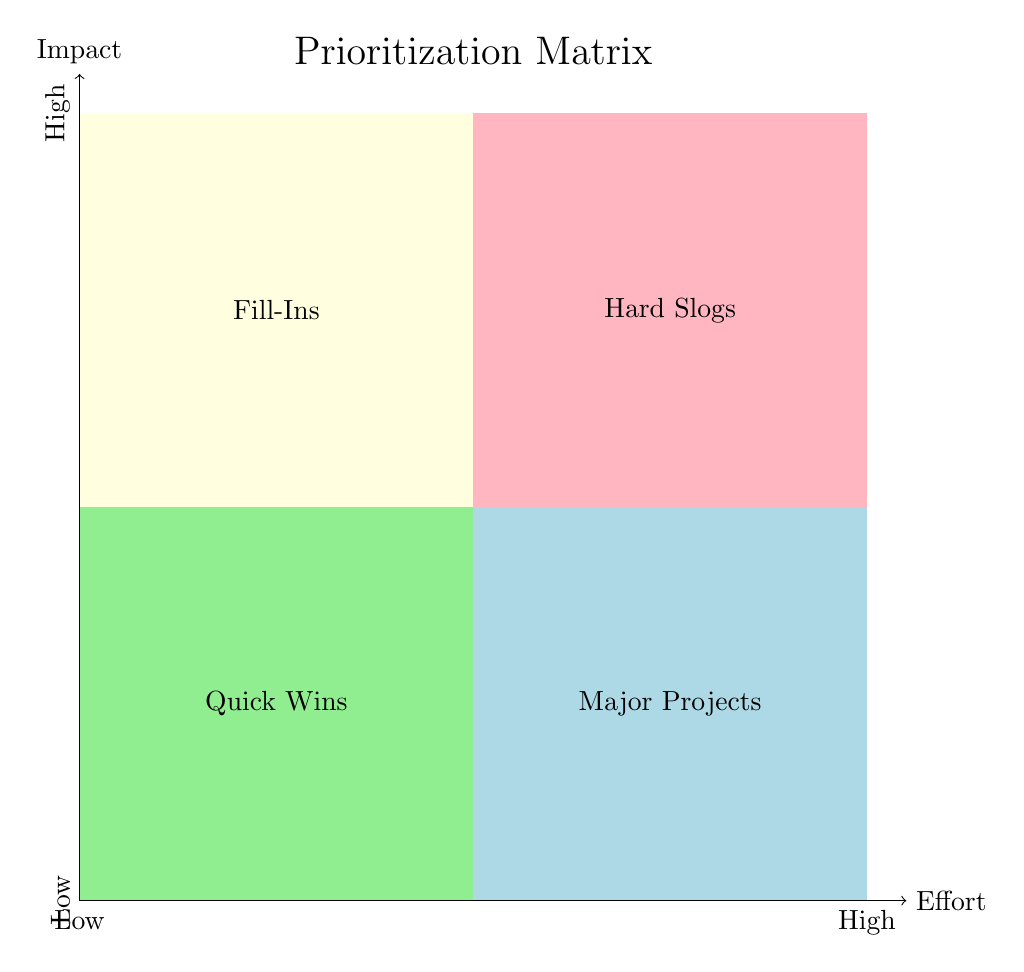
\begin{tikzpicture}
        % Define colors
    \definecolor{lightblue}{RGB}{173,216,230}
    \definecolor{lightgreen}{RGB}{144,238,144}
    \definecolor{lightyellow}{RGB}{255,255,224}
    \definecolor{lightred}{RGB}{255,182,193}

    % Draw the quadrants
    \fill[lightgreen] (0,0) rectangle (5,5);
    \fill[lightblue] (5,0) rectangle (10,5);
    \fill[lightyellow] (0,5) rectangle (5,10);
    \fill[lightred] (5,5) rectangle (10,10);

    % Draw the axes
    \draw[->] (0,0) -- (10.5,0) node[right] {Effort};
    \draw[->] (0,0) -- (0,10.5) node[above] {Impact};

    % Add labels to quadrants
    \node at (2.5,2.5) {Quick Wins};
    \node at (7.5,2.5) {Major Projects};
    \node at (2.5,7.5) {Fill-Ins};
    \node at (7.5,7.5) {Hard Slogs};

    % Add "Low" and "High" labels
    \node[below] at (0,0) {Low};
    \node[below] at (10,0) {High};
    \node[rotate=90, above] at (0,0) {Low};
    \node[rotate=90, above] at (0,10) {High};

    % Add a title
    \node[above] at (5,10.5) {\Large Prioritization Matrix};
\end{tikzpicture}

\subsection{Step 3: Select Technology Partners}

Based on your needs, choose the right tools. Consider:

1. \textbf{n8n for workflow automation}:
\begin{itemize}
    \item Open-source and self-hostable, providing full control over your data
    \item Highly flexible, allowing for complex workflow creation
    \item Cost-effective, with a free self-hosted option and reasonable cloud pricing
    \item Enables integration with a wide range of services and APIs
\end{itemize}

2. \textbf{NoCoDB for database management}:
\begin{itemize}
    \item Open-source alternative to Airtable, offering data sovereignty
    \item Provides a user-friendly interface for managing complex data
    \item Can be self-hosted, ensuring data privacy and reducing costs
    \item Allows for easy creation of views and forms for data entry
\end{itemize}

3. \textbf{BudiBase for creating custom applications}:
\begin{itemize}
    \item Open-source low-code platform, allowing for rapid application development
    \item Can be self-hosted, ensuring control over your applications and data
    \item Offers a range of pre-built components to speed up development
    \item Integrates well with various data sources, including NoCoDB
\end{itemize}

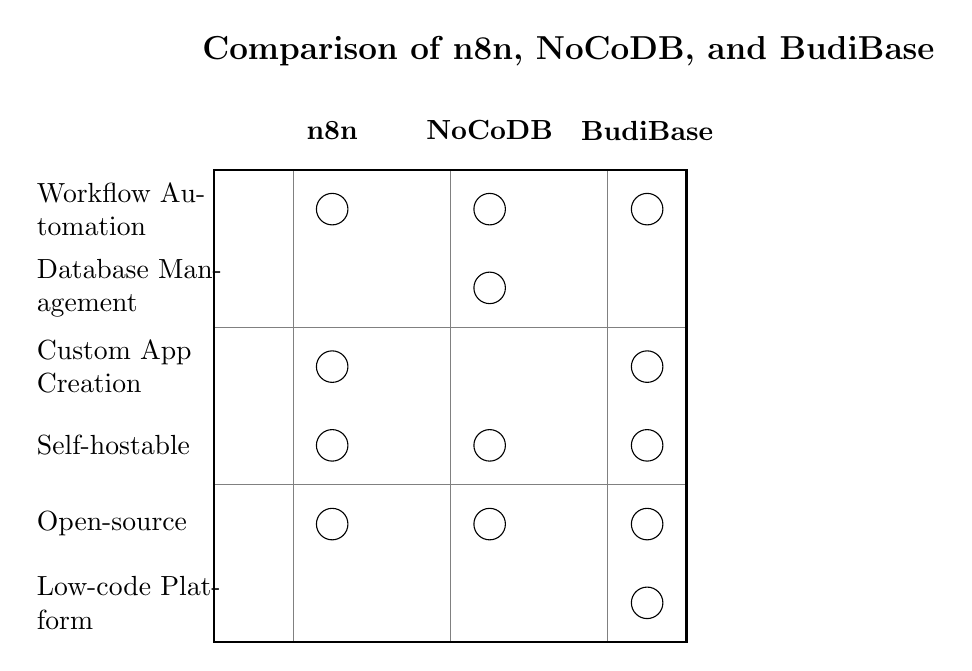
\begin{tikzpicture}[
    feature/.style={align=left, text width=2.5cm},
    tool/.style={align=center, font=\bfseries},
    check/.style={circle, draw, inner sep=0pt, minimum size=4mm, align=center},
    title/.style={font=\bfseries\large, align=center}
]

% Title
    \node[title] at (5.5, 5.5) {Comparison of n8n, NoCoDB, and BudiBase};

% Headers
    \node[tool] at (2.5, 4.5) {n8n};
    \node[tool] at (4.5, 4.5) {NoCoDB};
    \node[tool] at (6.5, 4.5) {BudiBase};

% Features
    \node[feature] at (0, 3.5) {Workflow Automation};
    \node[feature] at (0, 2.5) {Database Management};
    \node[feature] at (0, 1.5) {Custom App Creation};
    \node[feature] at (0, 0.5) {Self-hostable};
    \node[feature] at (0, -0.5) {Open-source};
    \node[feature] at (0, -1.5) {Low-code Platform};

% Checkmarks
    \foreach \x in {2.5, 4.5, 6.5} {
        \foreach \y in {3.5, 0.5, -0.5} {
            \node[check] at (\x, \y) {\checkmark};
        }
    }

    \node[check] at (2.5, 1.5) {\checkmark};
    \node[check] at (4.5, 2.5) {\checkmark};
    \node[check] at (6.5, 1.5) {\checkmark};
    \node[check] at (6.5, -1.5) {\checkmark};

% Draw grid
    \draw[step=2cm, gray, very thin] (1, -2) grid (7, 4);

% Border
    \draw[thick] (1, -2) rectangle (7, 4);

\end{tikzpicture}

\subsection{Step 4: Develop Your Solution}

When developing your automated solution:

1. \textbf{Start with a Minimum Viable Automation (MVA)}:
\begin{itemize}
    \item Focus on automating the core functionality first
    \item Aim for a working solution that can be tested and improved upon
    \item Get early feedback to guide further development
\end{itemize}

2. \textbf{Use modular design for scalability}:
\begin{itemize}
    \item Break down complex workflows into smaller, reusable components
    \item Design with future expansion in mind
    \item Use version control (e.g., Git) to manage your automation code
\end{itemize}

% TODO @screenshot: Example of a modular n8n workflow with reusable components

\subsection{Step 5: Test Rigorously}

Implement a comprehensive testing strategy:

1. \textbf{Unit testing for individual components}
2. \textbf{Integration testing for connected systems}
3. \textbf{User acceptance testing with your team}
4. \textbf{Performance and security testing}

\begin{tikzpicture}
    [
    node distance = 1.5cm and 3cm,
    box/.style = {rectangle, draw, rounded corners, minimum width=3cm, minimum height=1cm, align=center, fill=white},
    arrow/.style = {->, thick},
    cloud/.style = {ellipse, draw, minimum width=2cm, minimum height=1cm, align=center, fill=white},
    decision/.style = {diamond, draw, aspect=2, minimum width=2cm, align=center, fill=white}
    ]

% Nodes
    \node[cloud] (start) {Start};
    \node[box, below=of start] (unit) {Unit Testing};
    \node[box, below=of unit] (integration) {Integration Testing};
    \node[box, below=of integration] (user) {User Acceptance Testing};
    \node[box, below=of user] (performance) {Performance Testing};
    \node[box, below=of performance] (security) {Security Testing};
    \node[cloud, below=of security] (end) {End};

% Decision diamonds
    \node[decision, right=of unit] (unit_pass) {Pass?};
    \node[decision, right=of integration] (int_pass) {Pass?};
    \node[decision, right=of user] (user_pass) {Pass?};
    \node[decision, right=of performance] (perf_pass) {Pass?};
    \node[decision, right=of security] (sec_pass) {Pass?};

% Arrows
    \draw[arrow] (start) -- (unit);
    \draw[arrow] (unit) -- (unit_pass);
    \draw[arrow] (unit_pass) -- node[above, sloped] {Yes} (integration);
    \draw[arrow] (integration) -- (int_pass);
    \draw[arrow] (int_pass) -- node[above, sloped] {Yes} (user);
    \draw[arrow] (user) -- (user_pass);
    \draw[arrow] (user_pass) -- node[above, sloped] {Yes} (performance);
    \draw[arrow] (performance) -- (perf_pass);
    \draw[arrow] (perf_pass) -- node[above, sloped] {Yes} (security);
    \draw[arrow] (security) -- (sec_pass);
    \draw[arrow] (sec_pass) -- node[above, sloped] {Yes} (end);

% Feedback loops
    \draw[arrow] (unit_pass) -- node[above] {No} ++(-1.5,0) |- (unit);
    \draw[arrow] (int_pass) -- node[above] {No} ++(-1.5,0) |- (integration);
    \draw[arrow] (user_pass) -- node[above] {No} ++(-1.5,0) |- (user);
    \draw[arrow] (perf_pass) -- node[above] {No} ++(-1.5,0) |- (performance);
    \draw[arrow] (sec_pass) -- node[above] {No} ++(-1.5,0) |- (security);

% Title
    \node[above=0.5cm of start, font=\bfseries\large] {Comprehensive Testing Process for Automations};

\end{tikzpicture}

\subsection{Step 6: Deploy and Monitor}

1. \textbf{Gradual rollout}: Start with a pilot project or a subset of clients
2. \textbf{Continuous monitoring}: Use n8n to create monitoring workflows
3. \textbf{Feedback loop}: Regularly collect and act on user feedback

% TODO @screenshot: n8n workflow for monitoring automation performance

% TODO @template: Downloadable template for creating an automation roadmap


\section{Pricing and Packaging Automated Services}

Effectively monetizing your automated services is crucial for scaling your practice. Let's explore the best pricing strategies for small IT consulting firms.

\subsection{Top 3 Pricing Models for Automated Services}

1. \textbf{Tiered Subscription Model}
\begin{itemize}
    \item \textbf{Description}: Offer different levels of service (e.g., Basic, Pro, Enterprise)
    \item \textbf{Pros}: Predictable recurring revenue, easy upselling
    \item \textbf{Cons}: May leave money on the table with high-value clients
    \item \textbf{Example}: A consultant offers three tiers of automated reporting services, with higher tiers providing more frequent reports and custom dashboards
\end{itemize}

2. \textbf{Value-Based Pricing}
\begin{itemize}
    \item \textbf{Description}: Price based on the value delivered to the client
    \item \textbf{Pros}: Can lead to higher prices for high-impact automations
    \item \textbf{Cons}: Requires clear demonstration of ROI
    \item \textbf{Example}: Charging a percentage of the cost savings achieved through an automated inventory management system
\end{itemize}

3. \textbf{Hybrid Model: Base + Usage}
\begin{itemize}
    \item \textbf{Description}: Charge a base fee for setup and maintenance, plus usage-based fees
    \item \textbf{Pros}: Balances predictable income with scalability
    \item \textbf{Cons}: More complex to explain and implement
    \item \textbf{Example}: A fixed monthly fee for an automated customer support system, plus a per-ticket fee for issues resolved
\end{itemize}

\begin{tikzpicture}[
    node distance = 1cm and 0.5cm,
    box/.style = {rectangle, draw, rounded corners, minimum width=5cm, minimum height=1cm, align=center, fill=gray!20},
    title/.style = {font=\bfseries, align=center},
    pro/.style = {text=green!60!black, align=left},
    con/.style = {text=red!60!black, align=left}
]

% Title
    \node[title] at (0,0.5) {Comparison of Pricing Models};

% Headers
    \node[box] (TS) at (-5.5,-1) {Tiered Subscription};
    \node[box] (VB) at (0,-1) {Value-Based Pricing};
    \node[box] (HM) at (5.5,-1) {Hybrid: Base + Usage};

% Pros and Cons for Tiered Subscription
    \node[pro, below=0.5cm of TS.south west, anchor=north west, xshift=0.2cm, text width=4.8cm] (TS1) {+ Predictable revenue};
    \node[pro, below=0.2cm of TS1.south west, anchor=north west, text width=4.8cm] (TS2) {+ Easy upselling};
    \node[con, below=0.2cm of TS2.south west, anchor=north west, text width=4.8cm] (TS3) {- May undervalue high-impact work};

% Pros and Cons for Value-Based Pricing
    \node[pro, below=0.5cm of VB.south west, anchor=north west, xshift=0.2cm, text width=4.8cm] (VB1) {+ Higher prices for high impact};
    \node[pro, below=0.2cm of VB1.south west, anchor=north west, text width=4.8cm] (VB2) {+ Aligns with client value};
    \node[con, below=0.2cm of VB2.south west, anchor=north west, text width=4.8cm] (VB3) {- Requires clear ROI demonstration};

% Pros and Cons for Hybrid Model
    \node[pro, below=0.5cm of HM.south west, anchor=north west, xshift=0.2cm, text width=4.8cm] (HM1) {+ Balances predictability and scalability};
    \node[pro, below=0.2cm of HM1.south west, anchor=north west, text width=4.8cm] (HM2) {+ Flexible for various client needs};
    \node[con, below=0.2cm of HM2.south west, anchor=north west, text width=4.8cm] (HM3) {- More complex to explain};

% Vertical lines to separate columns
    \draw [gray] ($(TS.south east)+(0.25,0)$) -- ($(TS3.south east)+(0.25,0)$);
    \draw [gray] ($(VB.south east)+(0.25,0)$) -- ($(VB3.south east)+(0.25,0)$);

% Bounding box
    \node[draw, rounded corners, fit=(TS) (HM) (TS3) (HM3), inner sep=0.5cm] {};

\end{tikzpicture}

\subsection{Packaging Strategies}

Bundle automated services with traditional consulting to create compelling offers:

1. \textbf{The "Digital Transformation" Package}
\begin{itemize}
    \item Combine strategy consulting with implementation of key automations
    \item Offer ongoing support and optimization
\end{itemize}

2. \textbf{The "Efficiency Boost" Bundle}
\begin{itemize}
    \item Audit current processes and implement targeted automations
    \item Include training and change management support
\end{itemize}

3. \textbf{The "Scalability Suite"}
\begin{itemize}
    \item Focus on automations that enable client growth
    \item Tie pricing to client's growth metrics for alignment
\end{itemize}

\begin{tikzpicture}[
    package/.style={rectangle, draw, rounded corners, minimum width=4cm, minimum height=6cm, fill=gray!10},
    title/.style={font=\bfseries, align=center},
    item/.style={align=left, text width=3.5cm},
    icon/.style={circle, draw, minimum size=1cm, inner sep=0, font=\tiny\bfseries}
]

% Packages
    \node[package] (dt) at (0,0) {};
    \node[package] (eb) at (5,0) {};
    \node[package] (ss) at (10,0) {};

% Titles
    \node[title, above=0.2cm of dt.north] {Digital Transformation};
    \node[title, above=0.2cm of eb.north] {Efficiency Boost};
    \node[title, above=0.2cm of ss.north] {Scalability Suite};

% Digital Transformation items
    \node[item, above=0.5cm of dt.south] (dt1) {Strategy consulting};
    \node[item, above=0.5cm of dt1] (dt2) {Key automation implementation};
    \node[item, above=0.5cm of dt2] (dt3) {Ongoing support \& optimization};

% Efficiency Boost items
    \node[item, above=0.5cm of eb.south] (eb1) {Process audit};
    \node[item, above=0.5cm of eb1] (eb2) {Targeted automations};
    \node[item, above=0.5cm of eb2] (eb3) {Training \& change management};

% Scalability Suite items
    \node[item, above=0.5cm of ss.south] (ss1) {Growth-enabling automations};
    \node[item, above=0.5cm of ss1] (ss2) {Scalable infrastructure setup};
    \node[item, above=0.5cm of ss2] (ss3) {Growth-tied pricing model};

% Icons
    \node[icon] at (dt.north west) {DT};
    \node[icon] at (eb.north west) {EB};
    \node[icon] at (ss.north west) {SS};

% Connecting lines
    \draw[->] (dt1) -- ++(0.5,0);
    \draw[->] (dt2) -- ++(0.5,0);
    \draw[->] (dt3) -- ++(0.5,0);

    \draw[->] (eb1) -- ++(0.5,0);
    \draw[->] (eb2) -- ++(0.5,0);
    \draw[->] (eb3) -- ++(0.5,0);

    \draw[->] (ss1) -- ++(0.5,0);
    \draw[->] (ss2) -- ++(0.5,0);
    \draw[->] (ss3) -- ++(0.5,0);

% Title
    \node[font=\Large\bfseries] at (5,4) {Bundled Automation Packages};

\end{tikzpicture}


\section{Case Study: From 5 to 50 Clients with No Additional Hires}

Let's examine how one IT consulting practice leveraged automation to achieve 10x growth without expanding their team.

\subsection{The Challenge}

Our case study firm faced several challenges common to small IT consultancies:
\begin{itemize}
    \item Staying profitable while scaling
    \item Attracting new clients in a competitive market
    \item Pricing services competitively while maintaining margins
    \item Staying ahead of rapidly evolving tech trends
\end{itemize}

\subsection{The Automation Strategy}

The firm implemented a comprehensive automation strategy:

1. \textbf{Client Onboarding Automation}
\begin{itemize}
    \item Used n8n to create a seamless onboarding workflow
    \item Reduced onboarding time from 2 weeks to 2 days
\end{itemize}

2. \textbf{Automated Reporting and Analytics}
\begin{itemize}
    \item Developed custom dashboards using BudiBase
    \item Provided real-time insights to clients, improving satisfaction
\end{itemize}

3. \textbf{Predictive Maintenance Alerts}
\begin{itemize}
    \item Implemented IoT sensors and n8n workflows for client infrastructures
    \item Proactively addressed issues before they impacted clients
\end{itemize}

\begin{tikzpicture}
    [
    timeline/.style={
        ->,
        thick,
        draw=blue!50,
        line cap=round,
    },
    milestone/.style={
        circle,
        fill=blue!20,
        draw=blue,
        thick,
        inner sep=0pt,
        minimum size=24pt,
        font=\small\bfseries,
    },
    label/.style={
        text width=3.5cm,
        align=center,
        font=\small
    }
    ]

% Timeline
    \draw[timeline] (0,0) -- (14,0);

% Milestones
    \node[milestone] (start) at (0,0) {0};
    \node[milestone] (onboarding) at (3.5,0) {6};
    \node[milestone] (reporting) at (7,0) {12};
    \node[milestone] (maintenance) at (10.5,0) {15};
    \node[milestone] (end) at (14,0) {18};

% Labels
    \node[label, below=0.7cm of start] {Start:\\5 Clients};
    \node[label, above=0.7cm of onboarding] {Client Onboarding Automation};
    \node[label, below=0.7cm of onboarding] {Onboarding time reduced to 2 days};
    \node[label, above=0.7cm of reporting] {Automated Reporting \& Analytics};
    \node[label, below=0.7cm of reporting] {Real-time insights improve client satisfaction};
    \node[label, above=0.7cm of maintenance] {Predictive Maintenance Alerts};
    \node[label, below=0.7cm of maintenance] {Proactive issue resolution};
    \node[label, below=0.7cm of end] {End:\\50 Clients};

% Outcomes
    \node[anchor=north west, text width=14cm, align=left] at (0,4.5) {
        \textbf{Outcomes:}\\
        500\% revenue growth, 10x client base, NPS improved from 45 to 82, 40\% faster delivery
    };

% Time label
    \node[font=\small] at (7,-1.2) {Months};

% Title
    \node[font=\Large\bfseries] at (7,5.5) {Automation Journey: 5 to 50 Clients in 18 Months};

\end{tikzpicture}

\subsection{Measurable Outcomes}

The impact of these automations was significant:

1. \textbf{Revenue Growth}: 500% increase over 18 months
2. \textbf{Cost Reduction}: Maintained the same headcount while 10x-ing client base
3. \textbf{Client Satisfaction}: NPS score improved from 45 to 82
4. \textbf{Efficiency}: Reduced average project delivery time by 40%

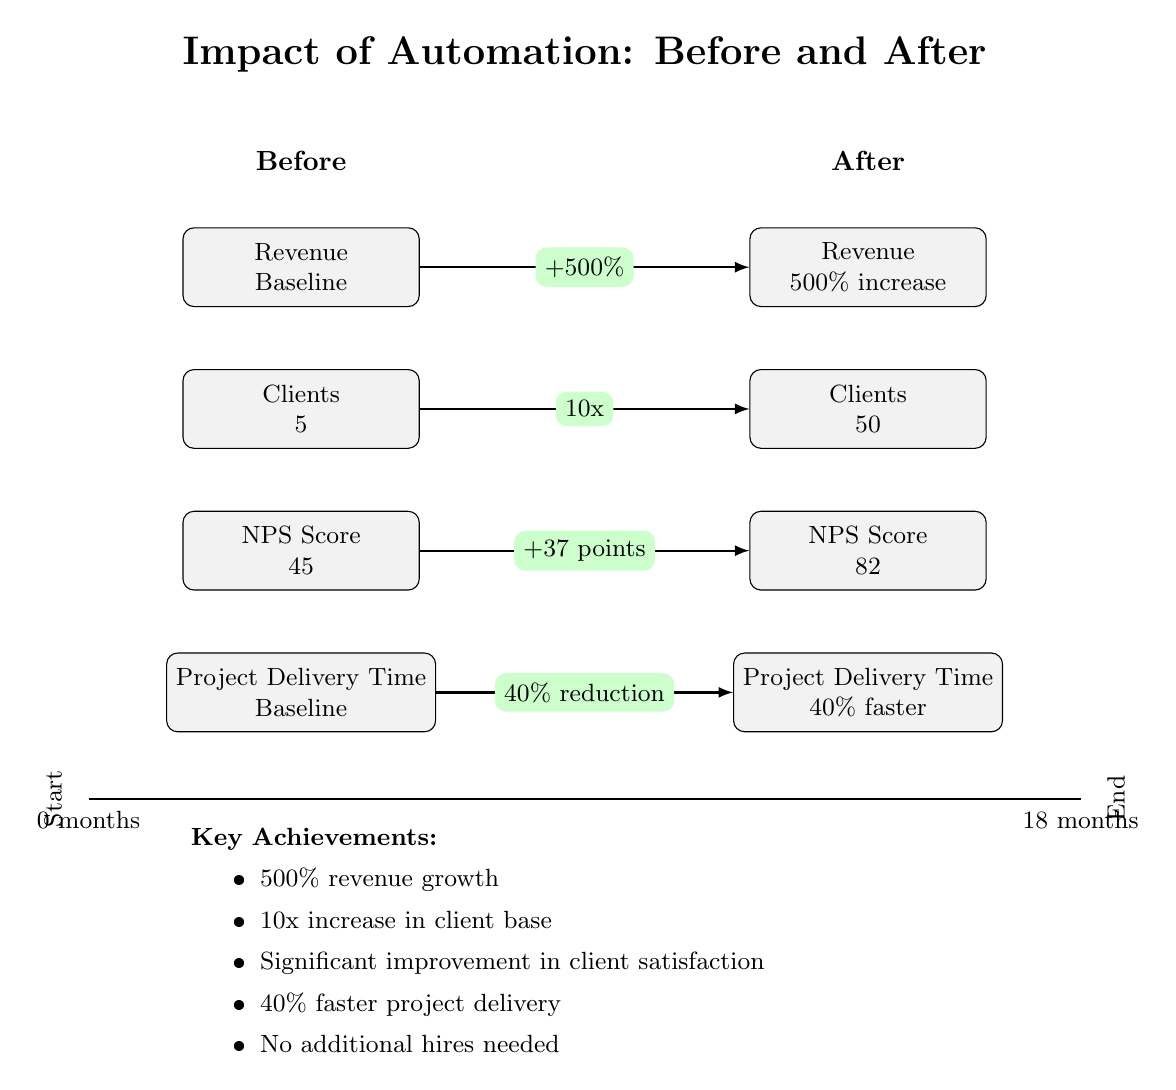
\begin{tikzpicture}
    [
    scale=0.9,
    every node/.style={font=\small},
    metric/.style={rectangle, rounded corners, draw, fill=gray!10, minimum width=3cm, minimum height=1cm, align=center},
    arrow/.style={->, >=latex, thick},
    label/.style={font=\bfseries}
    ]

% Title
    \node[font=\Large\bfseries] at (0,5) {Impact of Automation: Before and After};

% Before column
    \node[label] at (-4,3.5) {Before};
    \node[metric] (revenue_before) at (-4,2) {Revenue\\Baseline};
    \node[metric] (clients_before) at (-4,0) {Clients\\5};
    \node[metric] (nps_before) at (-4,-2) {NPS Score\\45};
    \node[metric] (efficiency_before) at (-4,-4) {Project Delivery Time\\Baseline};

% After column
    \node[label] at (4,3.5) {After};
    \node[metric] (revenue_after) at (4,2) {Revenue\\500\% increase};
    \node[metric] (clients_after) at (4,0) {Clients\\50};
    \node[metric] (nps_after) at (4,-2) {NPS Score\\82};
    \node[metric] (efficiency_after) at (4,-4) {Project Delivery Time\\40\% faster};

% Arrows
    \draw[arrow] (revenue_before) -- (revenue_after);
    \draw[arrow] (clients_before) -- (clients_after);
    \draw[arrow] (nps_before) -- (nps_after);
    \draw[arrow] (efficiency_before) -- (efficiency_after);

% Improvement labels
    \node[fill=green!20, rounded corners] at (0,2) {+500\%};
    \node[fill=green!20, rounded corners] at (0,0) {10x};
    \node[fill=green!20, rounded corners] at (0,-2) {+37 points};
    \node[fill=green!20, rounded corners] at (0,-4) {40\% reduction};

% Timeline
    \draw[thick] (-7,-5.5) -- (7,-5.5);
    \node at (-7,-5.8) {0 months};
    \node at (7,-5.8) {18 months};
    \node[rotate=90] at (-7.5,-5.5) {Start};
    \node[rotate=90] at (7.5,-5.5) {End};

% Key achievements
    \node[align=left, text width=10cm] at (0,-7.5) {
        \textbf{Key Achievements:}
        \begin{itemize}
            \item 500\% revenue growth
            \item 10x increase in client base
            \item Significant improvement in client satisfaction
            \item 40\% faster project delivery
            \item No additional hires needed
        \end{itemize}
    };

\end{tikzpicture}


\section{Overcoming Scaling Challenges}

As you scale your practice with automation, you may encounter several challenges:

1. \textbf{Data Management}: As your client base grows, managing and securing increasing amounts of data becomes crucial.
\begin{itemize}
    \item Solution: Implement robust data governance practices and leverage NoCoDB's advanced data management features.
\end{itemize}

2. \textbf{Maintaining Personal Touch}: Automation shouldn't come at the cost of personalized service.
\begin{itemize}
    \item Solution: Use n8n to create workflows that trigger personalized interactions at key points in the client journey.
\end{itemize}

3. \textbf{Keeping Up with Technology}: The rapid pace of technological change can be overwhelming.
\begin{itemize}
    \item Solution: Allocate time for continuous learning and experimentation with new tools and features.
\end{itemize}

4. \textbf{Managing Complexity}: As your automations grow, managing them can become complex.
\begin{itemize}
    \item Solution: Use modular design principles in n8n and maintain comprehensive documentation of your workflows.
\end{itemize}

\begin{tikzpicture}
    [
    scale=0.85,
    every node/.style={font=\small},
    challenge/.style={rectangle, rounded corners, draw=red!60, fill=red!10, minimum width=3cm, minimum height=1.5cm, align=center, text width=2.8cm},
    solution/.style={rectangle, rounded corners, draw=green!60, fill=green!10, minimum width=3cm, minimum height=2cm, align=center, text width=2.8cm},
    arrow/.style={->, >=latex, thick, draw=gray}
    ]

% Title
    \node[font=\Large\bfseries] at (0,6) {Common Scaling Challenges and Solutions};

% Challenges
    \node[challenge] (data) at (-6,3) {Data Management};
    \node[challenge] (personal) at (-2,3) {Maintaining Personal Touch};
    \node[challenge] (tech) at (2,3) {Keeping Up with Technology};
    \node[challenge] (complexity) at (6,3) {Managing Complexity};

% Solutions
    \node[solution] (data_sol) at (-6,0) {Implement robust data governance with NoCoDB};
    \node[solution] (personal_sol) at (-2,0) {Use n8n for personalized interaction triggers};
    \node[solution] (tech_sol) at (2,0) {Allocate time for continuous learning and experimentation};
    \node[solution] (complexity_sol) at (6,0) {Use modular design and maintain comprehensive documentation};

% Arrows
    \draw[arrow] (data) -- (data_sol);
    \draw[arrow] (personal) -- (personal_sol);
    \draw[arrow] (tech) -- (tech_sol);
    \draw[arrow] (complexity) -- (complexity_sol);

% Icons (using simple shapes as placeholders)
    \node[circle, fill=red!60, minimum size=0.8cm] at (-6,4) {\textcolor{white}{\faDatabase}};
    \node[circle, fill=red!60, minimum size=0.8cm] at (-2,4) {\textcolor{white}{\faUsers}};
    \node[circle, fill=red!60, minimum size=0.8cm] at (2,4) {\textcolor{white}{\faLaptopCode}};
    \node[circle, fill=red!60, minimum size=0.8cm] at (6,4) {\textcolor{white}{\faCogs}};

% Legend
    \node[draw, rectangle, rounded corners, fill=white, align=left, text width=4cm] at (0,-3) {
        \textbf{Legend:}
        \\ \textcolor{red!60}{\rule{0.5cm}{0.5cm}} Challenge
        \\ \textcolor{green!60}{\rule{0.5cm}{0.5cm}} Solution
    };

\end{tikzpicture}


\section{Conclusion}

Automation is not just a tool for efficiency; it's a catalyst for exponential growth in your IT consulting practice. By creating a thoughtful automation roadmap, pricing your services strategically, and learning from successful case studies, you can transform your practice and achieve remarkable scaling without proportionally increasing your workload or team size.

\textbf{Action Items}:
\begin{enumerate}
    \item Begin drafting your automation roadmap using the template provided.
    \item Choose one of the pricing models discussed and create a pricing structure for your automated services.
    \item Identify your top three processes to automate and outline the potential impact on your practice.
\end{enumerate}

% TODO @qr: QR code for downloading the Automation Planning Workbook

By taking these steps, you'll be well on your way to scaling your IT consulting practice through the power of automation. Remember, the journey of automation is ongoing - continually reassess, refine, and expand your automated processes to stay ahead in the ever-evolving world of IT consulting.